%%%%%%%%%%%%%%%%%%%%%%%%%%%%%%%%%%%%%%%%%%%%%%%%%%%%%%%%%%%%%%%%%%%%%%%%
\cleardoubleevenemptypage
\chapter{Introduction}
\label{ch:intro}
%%%%%%%%%%%%%%%%%%%%%%%%%%%%%%%%%%%%%%%%%%%%%%%%%%%%%%%%%%%%%%%%%%%%%%%%
\pgfmathsetmacro\chapclr{\colourarray[1]} % set the number to the chapter number. Yes, by hand. Don't ask me why.
\hypersetup{
  citecolor  = \chapclr,
  linkcolor  = \chapclr,
  urlcolor   = \chapclr,
}

\epigraph{
  A quasi-deep quote, with minimal relevance to the chapter.
  }{
    \textit{Piet J.M. Swinkels}
}

% The intro probably does not need an abstract:
% \begin{center}
%   \begin{minipage}{\abstractwidth\textwidth}
%     \begin{small}
%       Does the intro really need a short abstract?
%     \end{small}
%   \end{minipage}
%   \vspace{0.5cm}
% \end{center}
\clearpage
%%%%%%%%%%%%%%%%%%%%%%%%%%%%%%%%%%%%%%%%%%%%%%%%%%%%%%%%%%%%%%%%%%%%%%%%%%
\section{The first steps}
You know what are some really great papers? These: \cite{gabryelczykHydrogenBondGuidance2019,heesSelfassemblyOppositelyCharged2019,swinkelsRevealingPseudorotationRingopening2021}! Also, if I want to refer to an online video~\cite{ExampleVideo}, I can do that as well. By default, it will end up in a separate bibliography page! Neat! Look at Figure \ref{fig:ch1-dog}b! It is beautiful! 

\subsection{Continue with blind text}

\blindtext[2]
\subsection{Blahblah}
\blindtext[3]
Look at Figure \ref{fig:ch1-dog}b! It is beautiful! 

\begin{figure}
  \centering
  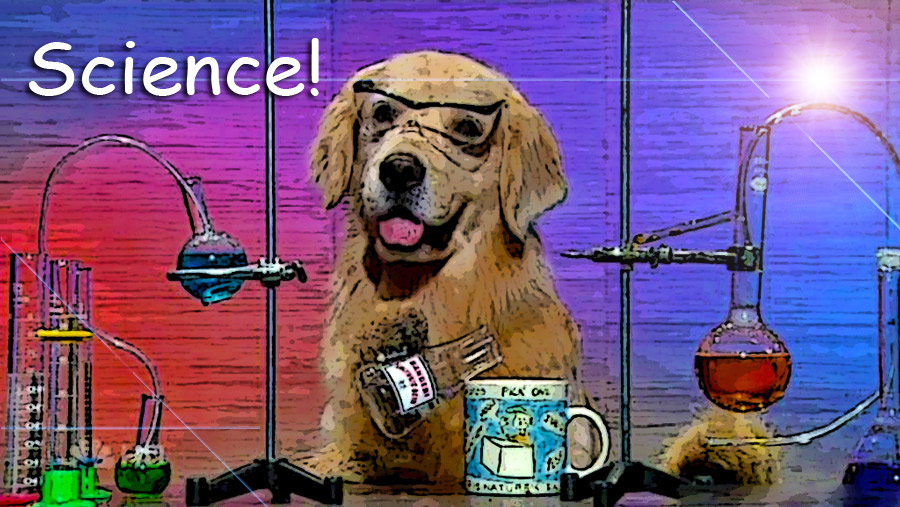
\includegraphics[width=1.0\linewidth]{Sections/Chapter1/Figures/dogs_do_science2.jpg}
  \caption{
    \textcolor{\chapclr}{Pure beauty.}
    I did something and I don't know how, and now I am writing that down somehow. Do you notice how the Figure caption is smaller than the main text, and that there is a small indentation on the left? You can change that! Also, the distance between this text and the main text can be controlled!
    }
  \label{fig:ch1-dog}
\end{figure}

\section{The second step}
\blindtext[1]
\subsection{More questions}
\blindtext[5]

